\subsection{Scaling in time and memory}
\label{sec:scaling}

\begin{figure}[tbp]
  \centering
  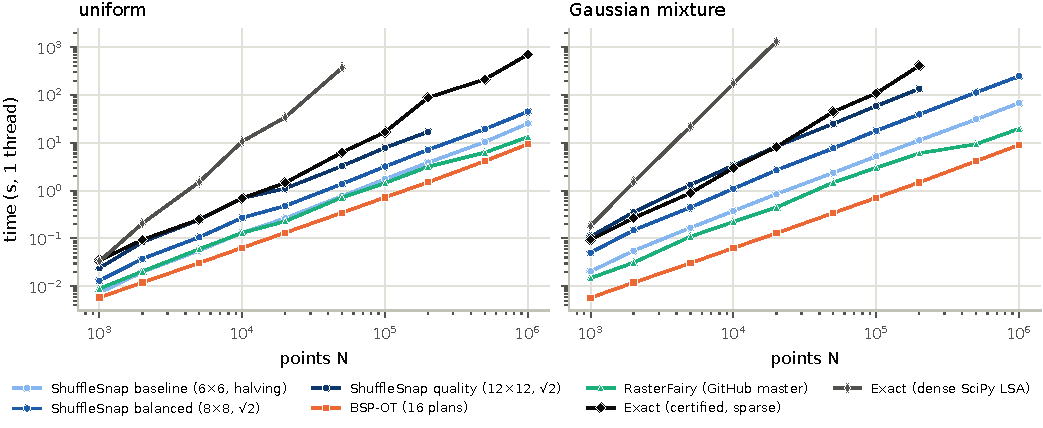
\includegraphics[width=\linewidth]{figures/fig_scaling.pdf}
  \caption{Time against $N$ on one thread (instance seed 1). Dense SciPy was run up to the
  largest size we considered sensible, 50k uniform points (6.2\,min, 23\,GiB) and 20k
  mixture points (22\,min). The certified solver was run up to $10^6$ uniform and
  $2\times10^5$ mixture points. The quality preset was run up to $2\times10^5$ points.}
  \label{fig:scaling}
\end{figure}

\begin{table}[tbp]
\centering\small
\caption{Peak extra resident memory (MiB) during one call, measured on a heap trimmed right
before the call (\texttt{malloc\_trim}), one thread, instance seed 1. Without trimming,
small allocations can reuse pages freed while the instance was generated and go unseen.}
\label{tab:memory}
\begin{tabular}{lrrrrrr}
\toprule
 & \multicolumn{3}{c}{uniform} & \multicolumn{3}{c}{Gaussian mixture} \\
method & $10^4$ & $10^5$ & $10^6$ & $10^4$ & $10^5$ & $10^6$ \\
\midrule
ShuffleSnap fast & 0.6 & 5.4 & 52.2 & 0.6 & 5.5 & 52.2 \\
ShuffleSnap balanced & 0.6 & 5.4 & 52.2 & 0.6 & 5.5 & 52.2 \\
ShuffleSnap quality & 0.6 & 5.4 & 52.2 & 0.6 & 5.5 & 52.2 \\
BSP-OT, 16 plans & 2.2 & 24.2 & 243 & 2.4 & 24.3 & 244 \\
RasterFairy master & 6.2 & 63.4 & 647 & 6.2 & 62.9 & 647 \\
exact, certified sparse & 49.5 & 437 & -- & 76.5 & 772 & -- \\
exact, dense SciPy & 1563 & -- & -- & 1564 & -- & -- \\
bisection only & 0.1 & 1.2 & 11.4 & 0.1 & 1.1 & 13.3 \\
\bottomrule
\end{tabular}

\end{table}

Between $10^4$ and $10^6$ points, \ShuffleSnap, BSP-OT and RasterFairy all scale close to
linearly. Their fitted exponents of time in $N$ are 1.15--1.18, 1.08 and about 1.0
(Figure~\ref{fig:scaling}). The time match with BSP-OT holds at $10^6$ uniform points: the fast
preset takes 9.8\,s on one core and BSP-OT with 16 plans 9.4\,s. The default takes 21\,s; with
24 threads, fast and default take 0.9\,s and 1.5\,s, and BSP-OT 2\,s. On the mixture, $10^6$
points take 14\,s (fast) and 43\,s (default) on one thread, or 1.0\,s and 2.7\,s on 24 threads.
RasterFairy takes 13--20\,s on one thread.

Exact solving scales worse but reaches further than we expected. The certified solver's
time grew as $N^{1.6}$ on uniform points and $N^{1.7}$ on the mixture. It certified $10^6$
uniform points in 11\,min using 4.2\,GiB, and $2\times10^5$ mixture points in 6.6\,min. Its
memory, 4--8\,kB per point, is set by the candidate edges and the flow solver. Dense SciPy
grew as $N^{2.2}$ (uniform) to $N^{2.9}$ (mixture) and needs $8N^2$ bytes. It took 6.2\,min
and 23\,GiB at 50k uniform points, and 22\,min at 20k mixture points. \ShuffleSnap\ needs
$O(N)$ working memory: an occupancy array, a position array, a last-change stamp per cell,
the window lists of the current level, and the input checks' temporary arrays. Measured,
this is 55--58 bytes per point at $10^5$ and $10^6$ points, or 52\,MiB at $10^6$
(Table~\ref{tab:memory}). The comparators need 4--12$\times$ more: BSP-OT about 250 and
RasterFairy about 670 bytes per point.

At $10^6$ uniform points, the quality ranking is unchanged. Measured against the certified
optimum of that instance, the excess is 3.3\% for fast, 1.3\% for the default and 0.58\% for
quality, against 74\% for BSP-OT (16 plans) and 48\% for RasterFairy. On uniform points the
default's excess grows with $N$: 0.11\% at $10^3$, 0.97\% at $10^5$ and 1.3\% at $10^6$ (one
instance each).

\paragraph{A billion points.} To see how far the method reaches beyond the benchmark, we solved
the largest instance of the earlier \ShuffleSnap\ work: 1{,}000{,}014{,}129 points of a 2D
random walk (the ``meander''), normalized to the unit square, on a $31{,}623\times31{,}623$
grid. We used the same random-permutation start, the default preset and 24 threads, on
the same workstation (Figure~\ref{fig:billion}). A dense cost matrix
would take 8\,EB. Setting up the start and the occupancy took 32\,s, and memory peaked at
53\,GiB, 57 bytes per point: coordinates and cell centers take 16 bytes each, change stamps
8, positions, occupancy and the grid index 4 each, and the window lists about 5. The kernel
accepts any mask; for a full rectangle, the centers and the index could be computed instead
of stored, which would save 20 of the 57 bytes. The walk is so concentrated that the result
moves the average point by about 6{,}900 cells (root mean square).

The default preset reached its fixed point after 1\,h\,43\,min (stride 1 began at
1\,h\,30\,min, and 78 stride-1 rounds followed). The coarse levels took about 4 minutes each,
because at this size nearly every window changes at every level and none can be skipped.
We then ran the quality preset's last four levels ($12\times12$ windows, strides 4 to 1),
which converged after 4.1\,h in total and lowered the cost by only $1.2\times10^{-6}$\%. Progress was front-loaded, as at smaller sizes: the cost
was within 1\% of the final one after 11 minutes, 0.1\% after 22, 0.01\% after 34 and 0.001\%
after 46, and after one hour it was only 0.0001\% above it.

No optimum is known for this instance, so we priced other assignments of the same instance on
the same frame. The earlier implementation ($6\times6$ windows, halving strides, 24 threads)
ran for six hours without converging. It reached stride 1 after 87 minutes and ended 0.0017\%
above our final cost, a level our run passed after 44 minutes. A memory-lean single-plan
port of BSP-OT, written for the earlier work because the official multi-plan code does not fit
in memory at this size, took 392\,s on one thread and is 8.2\% above. This is one instance
with no optimality certificate. It shows that the method runs to convergence at $10^9$ points
on one workstation, not how close it comes to the optimum there.

\begin{figure}[tbp]
  \centering
  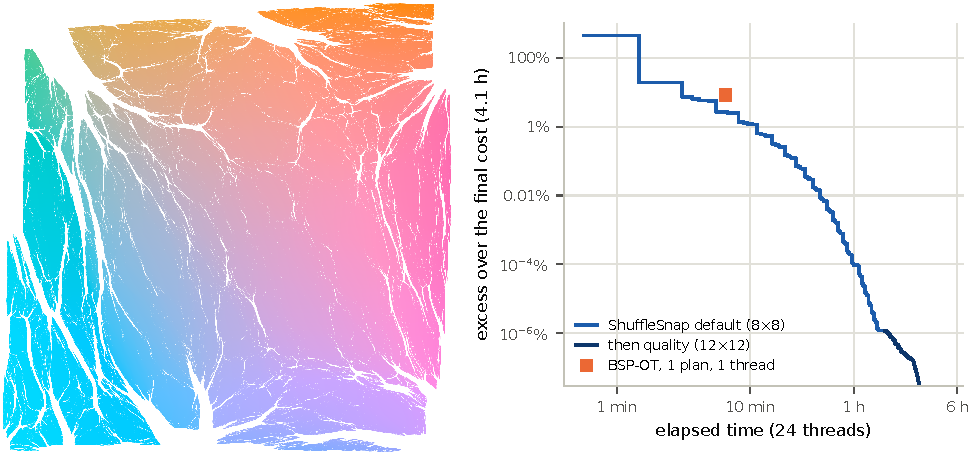
\includegraphics[width=\linewidth]{figures/fig_billion.pdf}
  \caption{A billion points. Left: every point drawn 75\% of the way from its
  input position to its assigned cell, one pixel per point, colored by input position and
  averaged over $10{,}000^2$ pixels (shown downsampled). White seams open where neighbouring
  cells hold points from distant sources; they follow the walk's folds. Right: cost after
  every phase as excess over the final cost: the default preset until its fixed point, then
  the quality preset's last four levels. A single-plan BSP-OT port is shown for comparison.}
  \label{fig:billion}
\end{figure}
